\documentclass[a4paper,11pt]{article}

\usepackage[utf8]{inputenc}
\usepackage[T1]{fontenc}
\usepackage[default]{lato}
\usepackage[margin=1.2cm, a4paper]{geometry}
\usepackage{xcolor}
\usepackage{graphicx}
\usepackage{tikz}
\usepackage{pgfplots}
\pgfplotsset{compat=1.18}
\usepackage{fontawesome5}
\usepackage{parskip}

\usetikzlibrary{calc, shapes, backgrounds, arrows.meta, positioning, shadings}

\hbadness=10000
\hfuzz=2pt

\definecolor{primary}{HTML}{0F4C81}
\definecolor{accent}{HTML}{E25A45}
\definecolor{secondary}{HTML}{F2B705}
\definecolor{graymid}{HTML}{7A7A7A}
\definecolor{bglight}{HTML}{F0F4F8}
\definecolor{bgdarker}{HTML}{B9D2E8}
\definecolor{heathigh}{HTML}{8B0000}
\definecolor{heatmid}{HTML}{FD8D3C}
\definecolor{heatlow}{HTML}{FFFACD}

\pagecolor{bglight}
\setlength{\parindent}{0pt}
\setlength{\parskip}{0pt}
\pagestyle{empty}

\begin{document}
	
	% ==========================================
	% HEADER (ANCHO COMPLETO)
	% ==========================================
	\noindent
	
\begin{tikzpicture}
		\fill[primary] (0,0) rectangle (\textwidth, -1.8);
		
		% Título a la izquierda
		\node[text=white, anchor=north west, font=\LARGE\bfseries] at (0.2, -0.3) {NYPD DATASET 2026};
		\node[text=bglight, anchor=north west, font=\normalsize] at (0.2, -1.0) {ANÁLISIS EXPLORATORIO DE DATOS (EDA)};
		
		% Metadatos a la derecha (alineados dentro del banner)
		\node[text=white, anchor=north east, align=left, font=\footnotesize] at (\textwidth-0.2cm, -0.35) {
			\faUniversity\ UBA - CEIA \hspace{12pt} \\
			\faUsers\ Grupo: 4  \\
			\faUsers\ Integrantes: Escobar, Mansilla, Kapobel \\
		};
	\end{tikzpicture}
	
	\vspace{0.4cm}
	
	% ==========================================
	% COLUMNA IZQUIERDA
	% ==========================================
	\noindent
	\begin{minipage}[t]{0.48\textwidth}
		\vspace{0pt}
		
		% Resumen en formato Tabla 
		\noindent
		\colorbox{white}{\parbox{\dimexpr\linewidth-2\fboxsep\relax}{
				\vspace{0.15cm}
				\renewcommand{\arraystretch}{1.3}
				\small
				\begin{tabular}{@{\hspace{0.1cm}} c p{1.7cm} p{4.8cm} @{}}
					\textcolor{primary}{\faDatabase} & \textbf{Volumen:} & 279.513 (279.5K) \\
					\textcolor{primary}{\faCalendar} & \textbf{Fecha:} & 1 Enero - 30 Junio 2026 \\
					\textcolor{primary}{\faMapMarker} & \textbf{Origen:} & New York - USA \\
					\textcolor{primary}{\faList} & \textbf{Variables:} & 36 ( 30 Categóricas, 6 Numéricas ) \\
					\textcolor{primary}{\faExclamationTriangle} & \textbf{Calidad:} & Presencia de datos incompletos como: \textit{'(null)'}, null y \textit{'UNKNOWN'} \\
				\end{tabular}
				\vspace{0.1cm}
		}}
		
		\vspace{0.4cm}
		
		\noindent
		\colorbox{primary}{\makebox[\dimexpr\linewidth-2\fboxsep\relax][l]{\textcolor{white}{\normalsize\textbf{\strut 2. DISTRIBUCIÓN DE GRAVEDAD DEL DELITO}}}}
		\vspace{0.1cm}
		
		\begin{center}
			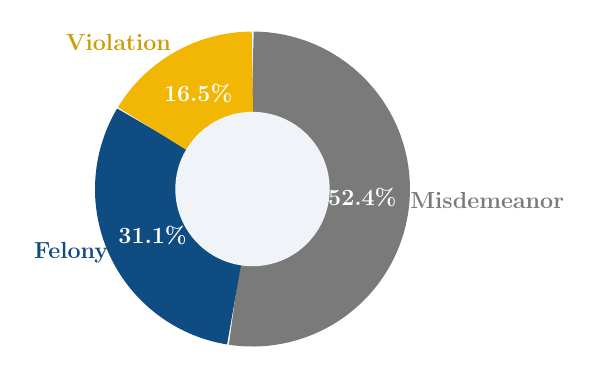
\begin{tikzpicture}[scale=0.7, transform shape]
				% Sectores del anillo
				\draw[graymid,   line width=12mm] (0,0) ++(90:2cm)   arc (90:-99:2cm);
				\draw[primary,   line width=12mm] (0,0) ++(-99:2cm)  arc (-99:-211:2cm);
				\draw[secondary, line width=12mm] (0,0) ++(-211:2cm) arc (-211:-270:2cm);
				\fill[bglight] (0,0) circle (1.4cm);
				
				% Porcentajes dentro del anillo (blanco)
				\node[white, font=\large\bfseries] at (-4.5:2cm)   {52.4\%};
				\node[white, font=\large\bfseries] at (-155:2cm)   {31.1\%};
				\node[white, font=\large\bfseries] at (119.5:2cm)  {16.5\%};
				
				% Nombres fuera del anillo
				\node[graymid,   font=\large\bfseries, anchor=west]        at (-4.5:2.75cm)  {Misdemeanor};
				\node[primary,   font=\large\bfseries, anchor=east]        at (-155:2.75cm)  {Felony};
				\node[secondary!85!black, font=\large\bfseries, anchor=south east] at (119.5:2.75cm) {Violation};
			\end{tikzpicture}
		\end{center}
		
		\vspace{0.3cm}
		
		% ---------- MAPA DE CALOR: DÍA VS HORA ----------
		\noindent
		\colorbox{primary}{\makebox[\dimexpr\linewidth-2\fboxsep\relax][l]{\textcolor{white}{\normalsize\textbf{\strut 3. CONCENTRACIÓN: DÍA VS HORA}}}}
		\vspace{0.1cm}
		
		\begin{center}
			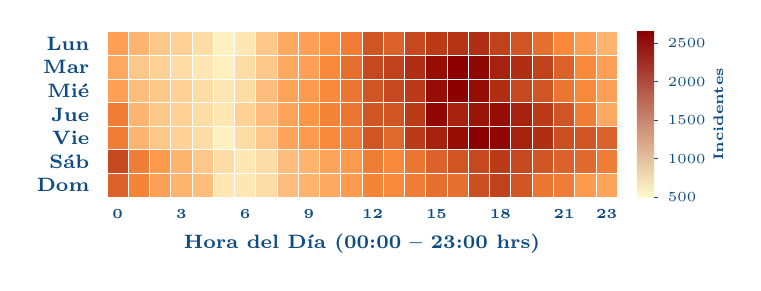
\begin{tikzpicture}
				\def\cw{0.27}
				\def\ch{0.30}
				
				\foreach \val [count=\i from 0] in {
					1400,1200,1000,900,800,600,700,1000,1300,1400,1500,1700,2000,1900,2100,2200,2250,2300,2150,2000,1800,1600,1400,1200,
					1300,1000,900,800,700,600,800,1000,1300,1400,1600,1800,2100,2150,2300,2550,2650,2600,2400,2300,2150,1900,1600,1400,
					1400,1100,1000,900,800,700,800,1100,1350,1450,1600,1750,2000,2100,2200,2550,2650,2550,2300,2100,2000,1750,1600,1400,
					1700,1200,1000,900,800,700,900,1100,1350,1500,1650,1750,2000,2000,2200,2600,2400,2500,2550,2400,2200,2000,1700,1300,
					1700,1200,1000,900,800,600,800,1000,1350,1450,1600,1700,2000,1850,2200,2400,2550,2650,2600,2400,2300,2050,2000,1900,
					2100,1700,1450,1200,1000,800,700,800,1100,1200,1350,1450,1700,1600,1750,1900,2000,2100,2200,2100,2000,1900,1850,1700,
					1900,1650,1400,1200,1100,700,700,800,1100,1200,1300,1450,1650,1600,1700,1800,1800,2050,2150,2000,1750,1700,1450,1350} {
					\pgfmathtruncatemacro{\hx}{mod(\i,24)}
					\pgfmathtruncatemacro{\dy}{int(\i/24)}
					\pgfmathsetmacro{\aa}{max(0,min(100,(\val-500)/21.5))}
					\ifdim\aa pt<50pt
					\pgfmathsetmacro{\bb}{\aa*2}
					\colorlet{cc}{heatmid!\bb!heatlow}
					\else
					\pgfmathsetmacro{\bb}{(\aa-50)*2}
					\colorlet{cc}{heathigh!\bb!heatmid}
					\fi
					\fill[cc, draw=white, line width=0.3pt] (\hx*\cw, -\dy*\ch) rectangle ++(\cw, -\ch);
				}
				
				\foreach \dd [count=\y from 0] in {Lun, Mar, Mié, Jue, Vie, Sáb, Dom} {
					\node[anchor=east, font=\scriptsize\bfseries, text=primary] at (-0.1, -\y*\ch - 0.5*\ch) {\dd};
				}
				
				\foreach \hh in {0, 3, 6, 9, 12, 15, 18, 21, 23} {
					\node[anchor=north, font=\tiny\bfseries, text=primary] at (\hh*\cw + 0.5*\cw, -7*\ch - 0.03) {\hh};
				}
				\node[anchor=north, font=\scriptsize\bfseries, text=primary] at (12*\cw, -7*\ch - 0.35) {Hora del Día (00:00 -- 23:00 hrs)};
				
				\pgfmathsetmacro{\cbx}{24*\cw + 0.25}
				\pgfmathsetmacro{\cbh}{7*\ch}
				\shade[bottom color=heatlow, middle color=heatmid, top color=heathigh]
				(\cbx, 0) rectangle ++(0.22, -\cbh);
				\foreach \tv in {500,1000,1500,2000,2500} {
					\pgfmathsetmacro{\ty}{-\cbh + (\tv-500)/2150*\cbh}
					\draw[primary, line width=0.3pt] (\cbx+0.22, \ty) -- ++(0.05,0);
					\node[anchor=west, font=\tiny, text=primary] at (\cbx+0.27, \ty) {\tv};
				}
				\node[font=\tiny\bfseries, text=primary, rotate=90, anchor=north] at (\cbx+0.85, -0.5*\cbh) {Incidentes};
			\end{tikzpicture}
		\end{center}
		\vspace{-0.1cm}
		\raggedright
		\footnotesize \textit{Hallazgo: Alta concentración de incidentes de martes a viernes entre las 15:00 y 19:00 hrs.}
		
	\end{minipage}%
	\hfill
	% ==========================================
	% COLUMNA DERECHA
	% ==========================================
	\begin{minipage}[t]{0.48\textwidth}
		\vspace{0pt}
		
		\noindent
		\colorbox{primary}{\makebox[\dimexpr\linewidth-2\fboxsep\relax][l]{\textcolor{white}{\normalsize\textbf{\strut 1. DIFICULTADES Y FEATURES CLAVE}}}}
		\vspace{0.1cm}
		
		\noindent
		\colorbox{white}{\parbox{\dimexpr\linewidth-2\fboxsep\relax}{
				\vspace{0.08cm}
				\scriptsize
				\setlength{\leftmargini}{1.1em}
				
				\textcolor{primary}{\textbf{Dificultades}}\par
				\begin{itemize}
					\setlength{\itemsep}{0.04cm}
					\setlength{\topsep}{0.04cm}
					\setlength{\parsep}{0pt}
					\item \textbf{Datos faltantes:} \textit{(null)}, null y \textit{UNKNOWN} requieren criterios por variable. Por ejemplo:
					\subitem \textit{HADEVELOPT} (Nombre del complejo de la Autoridad de Vivienda donde ocurrió el hecho) posee 279.5k valores \textit{(null)}.
					\subitem \textit{TRANSIT\_DISTRICT} (Distrito de tránsito en el que ocurrió el delito) posee 261.7k valores nulos reales.
					\item \textbf{Edades:} Sospechosos y víctimas están agrupados en rangos categóricos; hay que normalizar valores desconocidos o inválidos.
					\item \textbf{ML:} El dataset no tiene un target explícito; la tarea y la variable objetivo deben definirse.
				\end{itemize}
				
				\vspace{0.3cm}
				\textcolor{primary}{\textbf{Features destacadas}}\par
				\begin{itemize}
					\setlength{\itemsep}{0.04cm}
					\setlength{\topsep}{0.04cm}
					\setlength{\parsep}{0pt}
					\item \textbf{Clasificación por gravedad:} \texttt{LAW\_CAT\_CD} distingue felony, misdemeanor y violation.
					\item \textbf{Clasificación por tipo:} \texttt{KY\_CD}/\texttt{OFNS\_DESC} clasificación del delito y su descricipción; \texttt{PD\_CD}/\texttt{PD\_DESC} igual pero más granular.
					\item \textbf{Ubicación:} \texttt{BORO\_NM} permite agrupar por ciudad; hay X/Y State Plane, latitud/longitud WGS84 y campos georreferenciados compuestos. \texttt{PREM\_TYP\_DESC} permite saber obtener una descripción del lugar físico del hecho.
					\item \textbf{Tiempo:} \texttt{CMPLNT\_FR\_DT/TM} indica ocurrencia; \texttt{RPT\_DT}, la fecha de reporte.
				\end{itemize}
				\vspace{0.04cm}
		}}
		
		\vspace{0.3cm}
		
		% ---------- TENDENCIA MENSUAL ----------
		\noindent
		\colorbox{primary}{\makebox[\dimexpr\linewidth-2\fboxsep\relax][l]{\textcolor{white}{\normalsize\textbf{\strut 4. TENDENCIA MENSUAL DE INCIDENTES}}}}
		\vspace{0.5cm}
		
		\begin{center}
			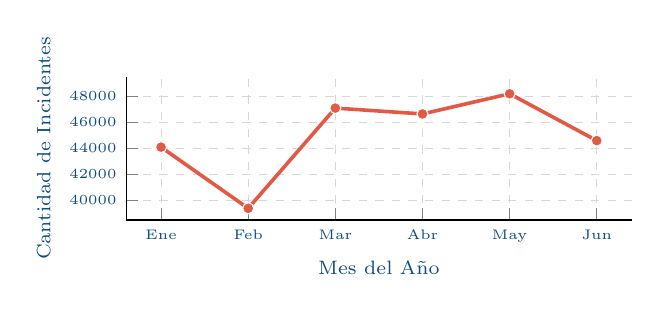
\begin{tikzpicture}
				\begin{axis}[
					width=8cm,
					height=3.4cm,
					xlabel={Mes del Año},
					ylabel={Cantidad de Incidentes},
					xlabel style={font=\scriptsize, text=primary},
					ylabel style={font=\scriptsize, text=primary},
					xtick={1,2,3,4,5,6},
					xticklabels={Ene,Feb,Mar,Abr,May,Jun},
					xticklabel style={font=\tiny, text=primary},
					ymin=38500, ymax=49500,
					xmin=0.6, xmax=6.4,
					ytick={40000,42000,44000,46000,48000},
					scaled y ticks=false,
					yticklabel style={font=\tiny, text=primary},
					yticklabel={\pgfmathprintnumber[fixed,precision=0,1000 sep={}]{\tick}},
					grid=both,
					grid style={dashed, graymid!30},
					axis lines*=left,
					]
					\addplot[
					color=accent,
					line width=1.3pt,
					mark=*,
					mark size=2pt,
					mark options={fill=accent, draw=white, line width=0.4pt},
					] coordinates {
						(1,44100) (2,39400) (3,47100) (4,46650) (5,48200) (6,44600)
					};
				\end{axis}
			\end{tikzpicture}
		\end{center}
		\vspace{-0.1cm}
		\raggedright
		\footnotesize \textit{Hallazgo: Mayo registra el mayor volumen de incidentes y febrero el menor.}
		
	\end{minipage}
	
	\vspace{0.3cm}
	
	% ==========================================
	% GRÁFICO A ANCHO COMPLETO
	% ==========================================
	\noindent
	\colorbox{primary}{\makebox[\dimexpr\textwidth-2\fboxsep\relax][l]{\textcolor{white}{\normalsize\textbf{\strut 5. GRAVEDAD SEGÚN ENTORNO (TOP 10)}}}}
	
	\begin{center}
		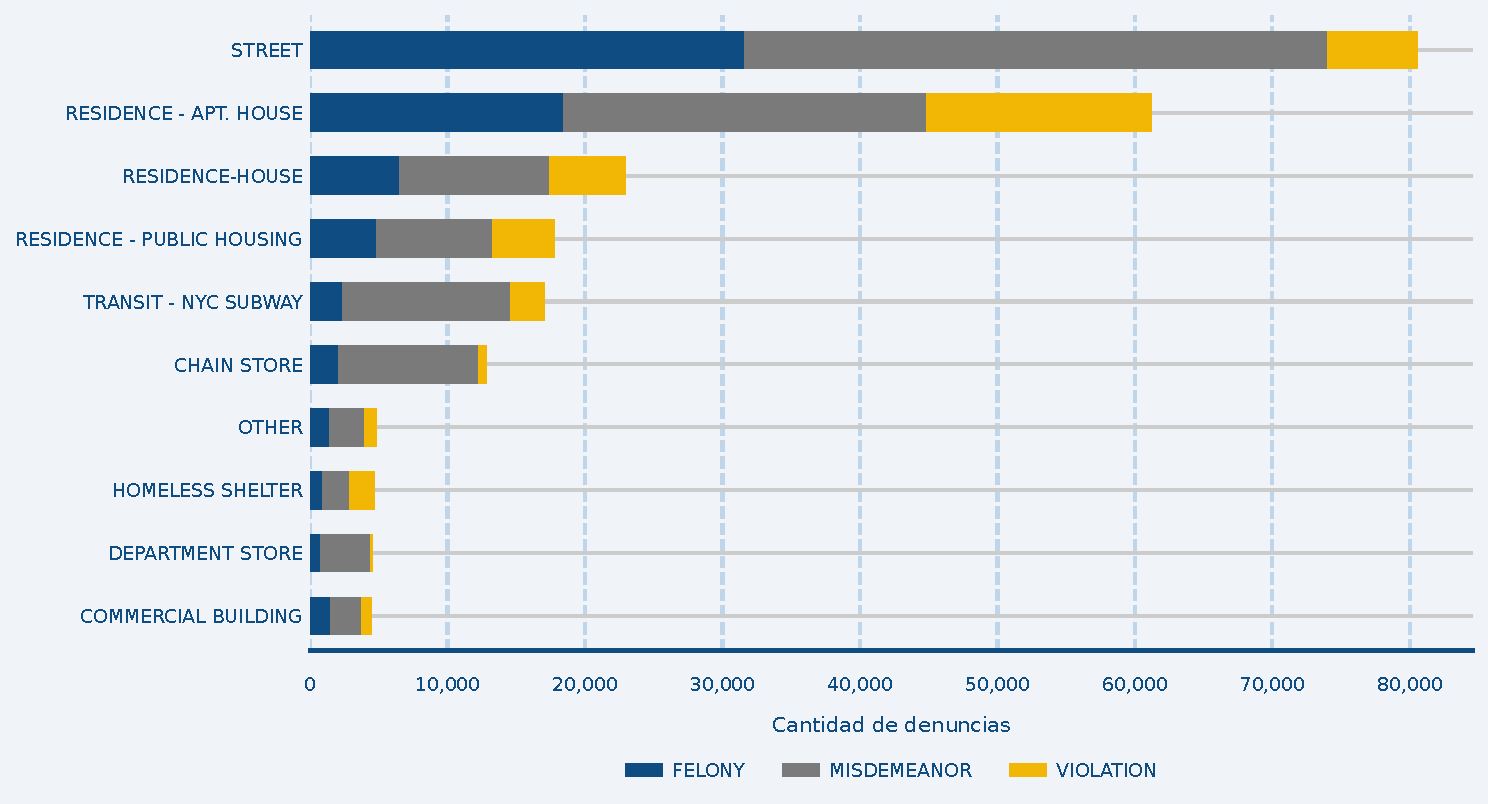
\includegraphics[width=\linewidth, height=6.5cm, keepaspectratio]{images/gravedad_entorno.pdf}
	\end{center}
	
	\vspace{-0.3cm}
	\noindent
	\footnotesize \textit{Nota: Top 10 categorías de entorno físico con mayor volumen de reportes.}

	\newpage
	\vspace{0.3cm}
	
	\noindent
	\colorbox{primary}{\makebox[\dimexpr\textwidth-2\fboxsep\relax][l]{\textcolor{white}{\normalsize\textbf{\strut 6. DENSIDAD ESPACIAL POR GRAVEDAD Y JURISDICCIÓN}}}}
	\vspace{0.3cm}
	
	\begin{center}
		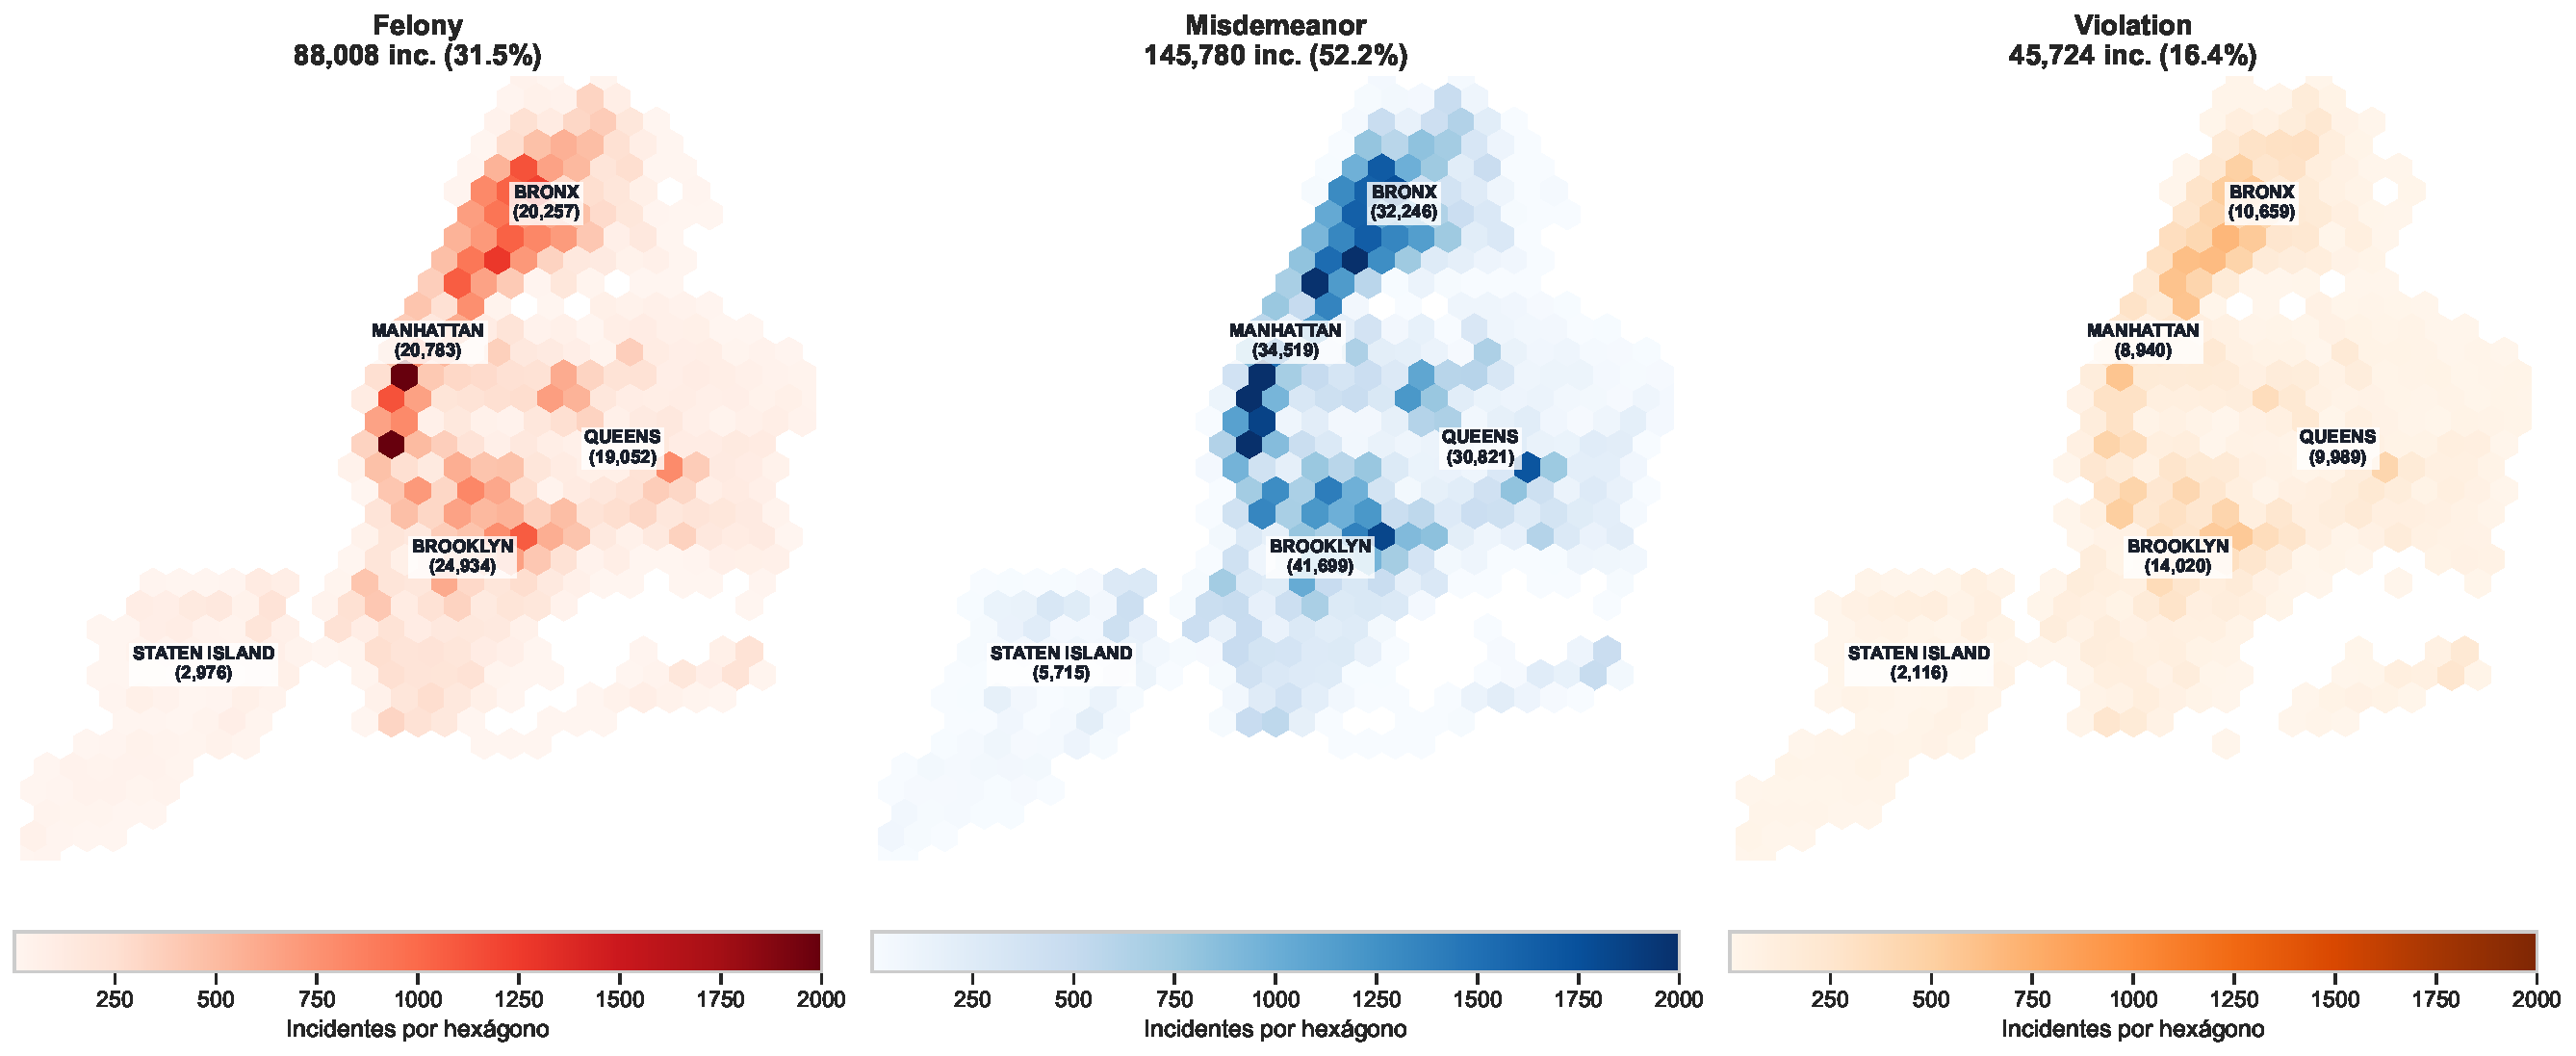
\includegraphics[width=\linewidth, height=15cm, keepaspectratio]{images/mapa_espacial_gravedad_1.pdf}
	\end{center}
	
	\vspace{0.3cm}
	\noindent
	\footnotesize \textit{Hallazgo: En las tres gravedades los focos se concentran en Manhattan y el Bronx. Misdemeanor es la categoría con mayor volumen y con los hexágonos más densos.}
	
\end{document}
